\section{Issuer}

\subsection{Registrazione}
In questa sezione un utente può registarsi inserendo \textbf{Email} e \textbf{Password} valide. Una volta registrato l'utente riceverà un messaggio di conferma e verrà reindirizzato alla pagina \textbf{Home}.
\begin{center}
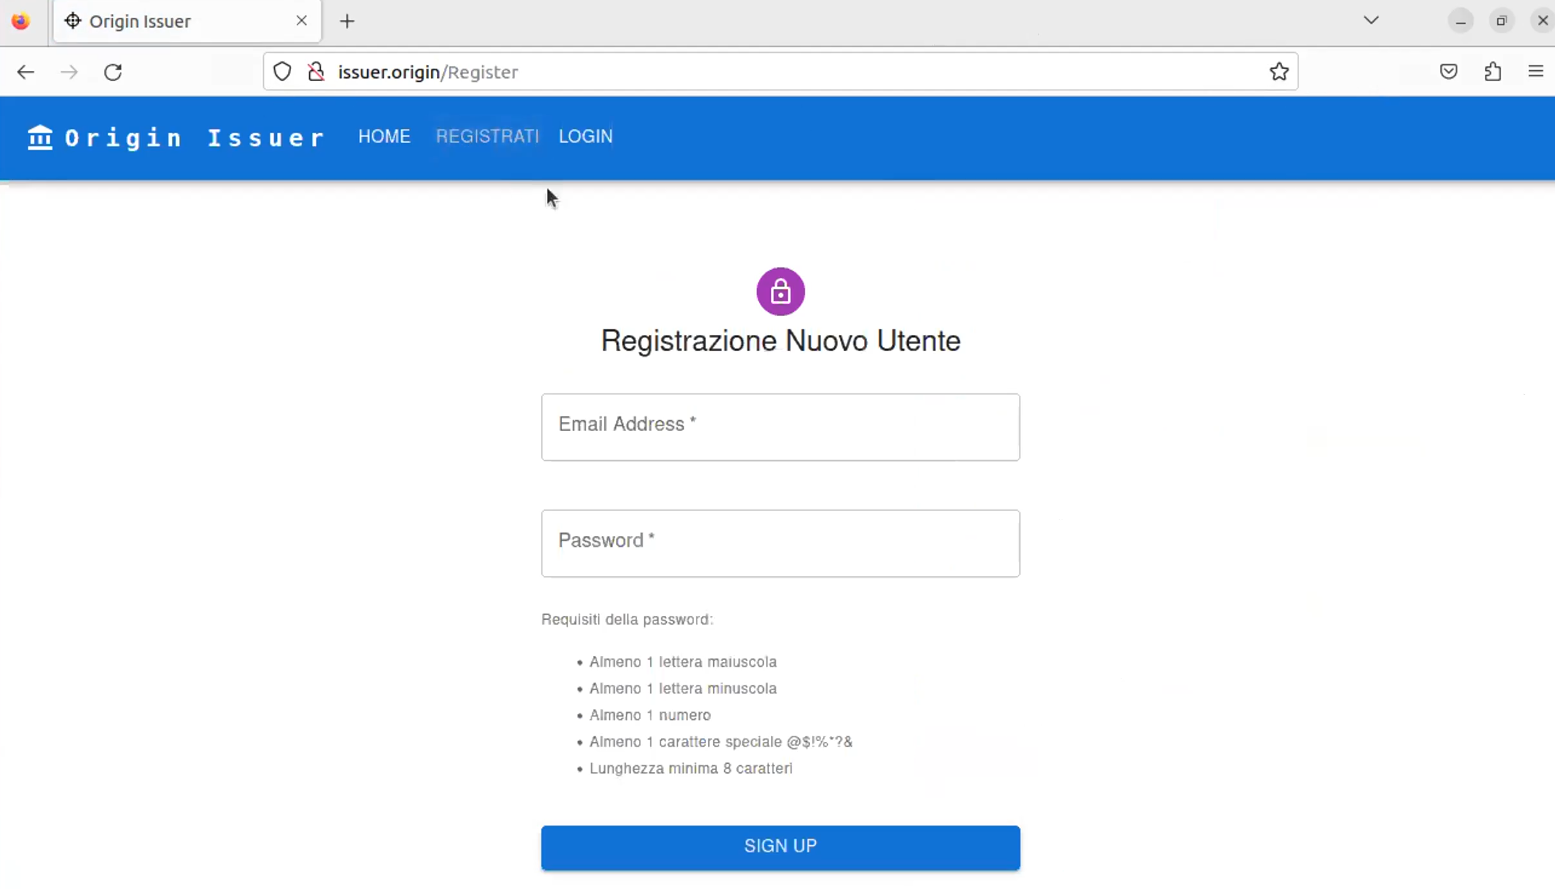
\includegraphics[scale = 0.2]{./res/img/issuer/new/registrazione.png}
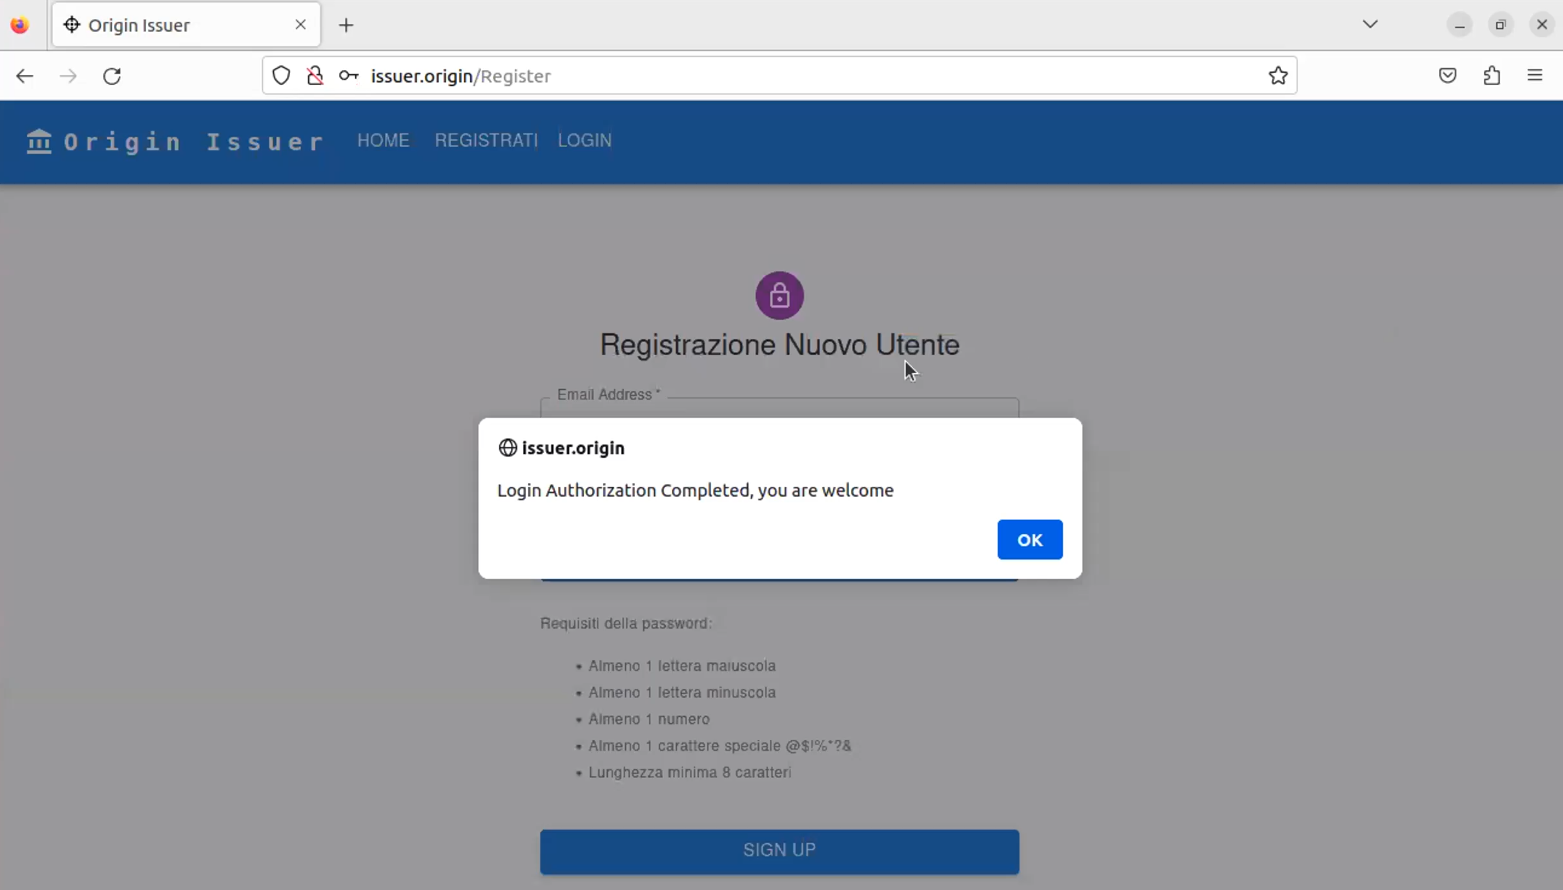
\includegraphics[scale = 0.2]{./res/img/issuer/new/registrazione2.png}
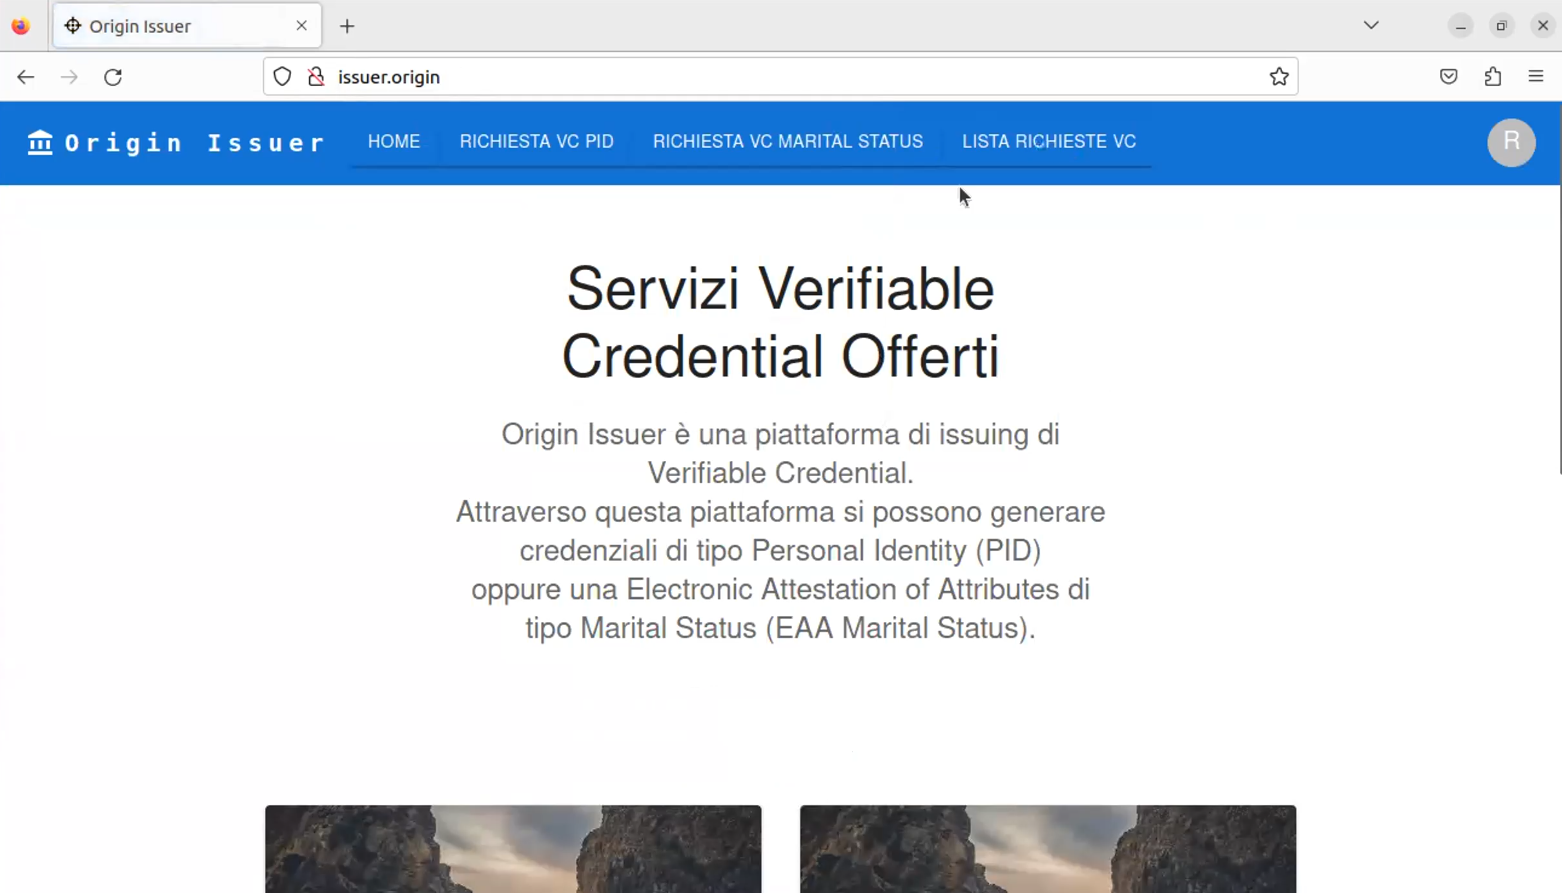
\includegraphics[scale = 0.2]{./res/img/issuer/new/registrazione3.png}
\end{center}

\subsection{Login}
\subsubsection{Login utente}
In questa pagina un \textbf{utente} può effettuare il login inserendo \textbf{Email} e \textbf{Password} valide. Una volta effettuato il login l'utente verrà reindirizzato alla sua pagina \textbf{Home}.
\begin{center}
    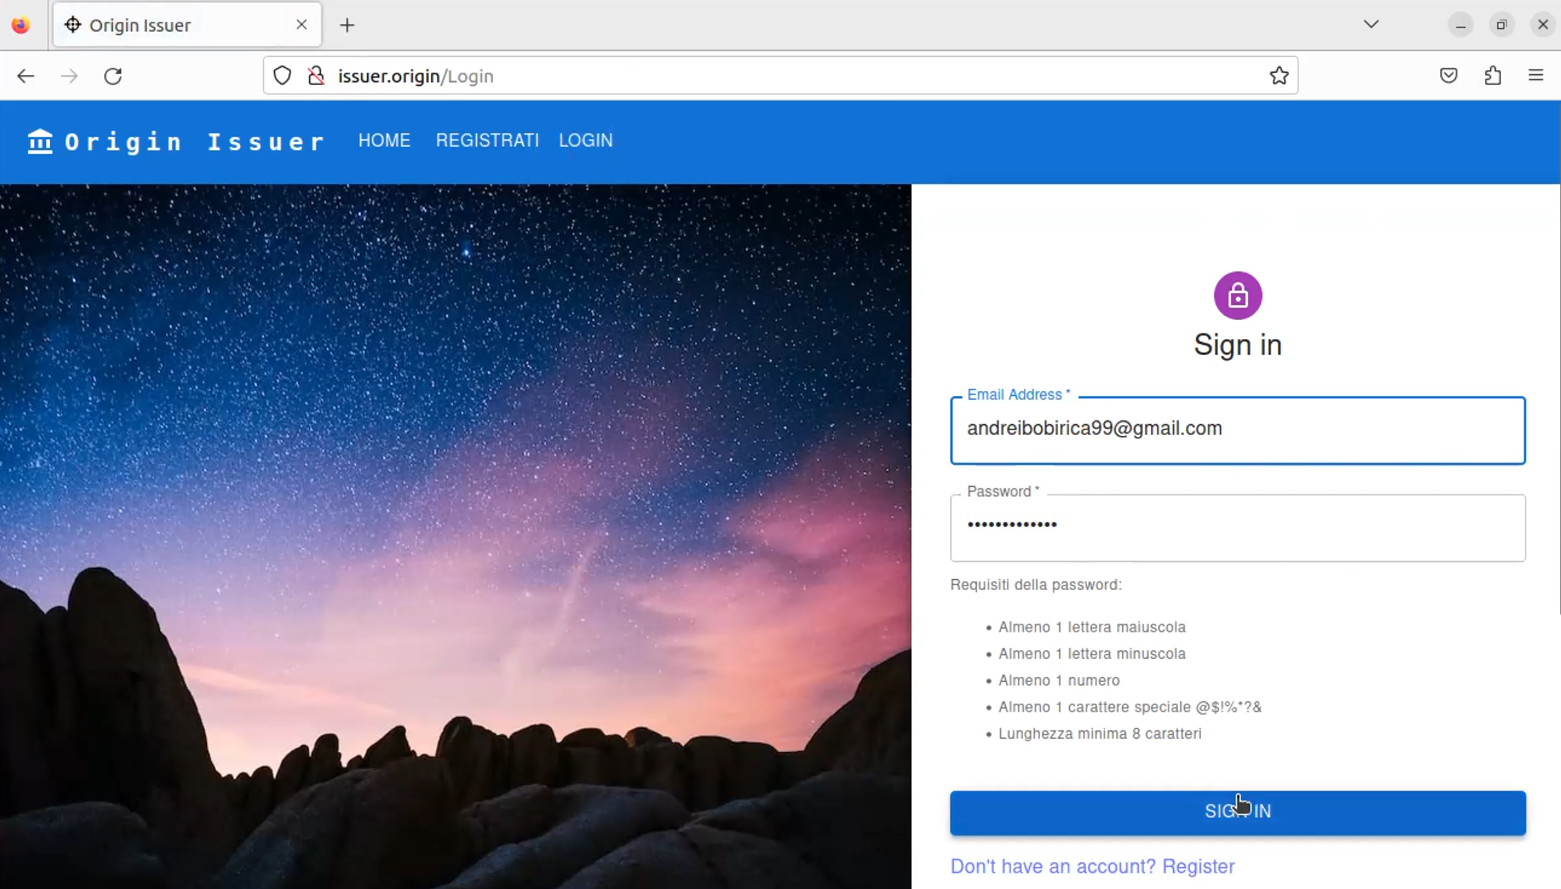
\includegraphics[scale = 0.2]{./res/img/issuer/new/login1.png}
    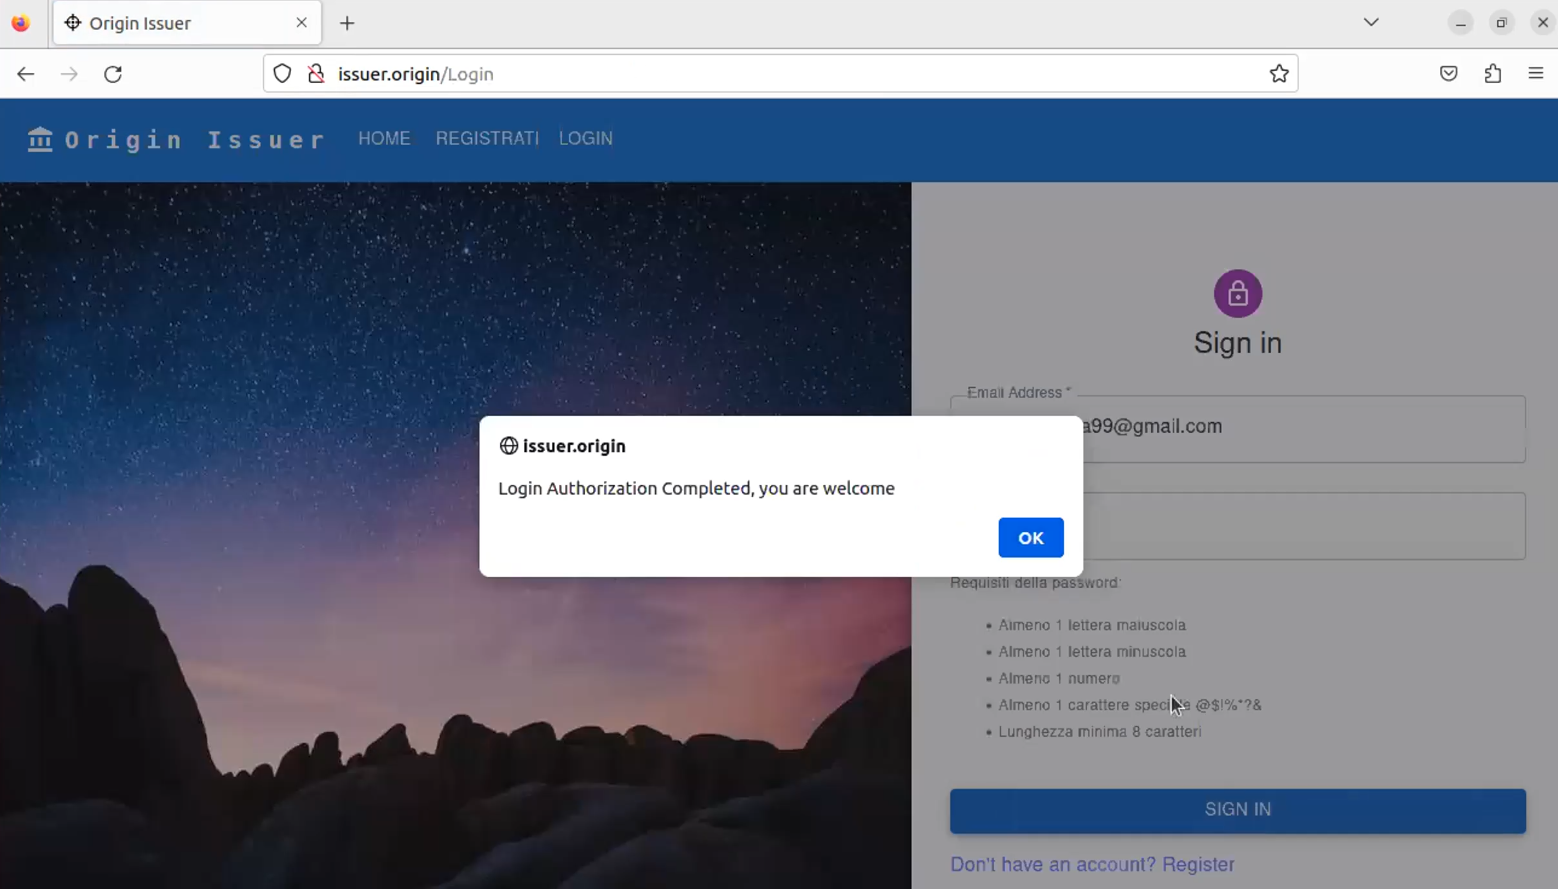
\includegraphics[scale = 0.2]{./res/img/issuer/new/login2.png}
    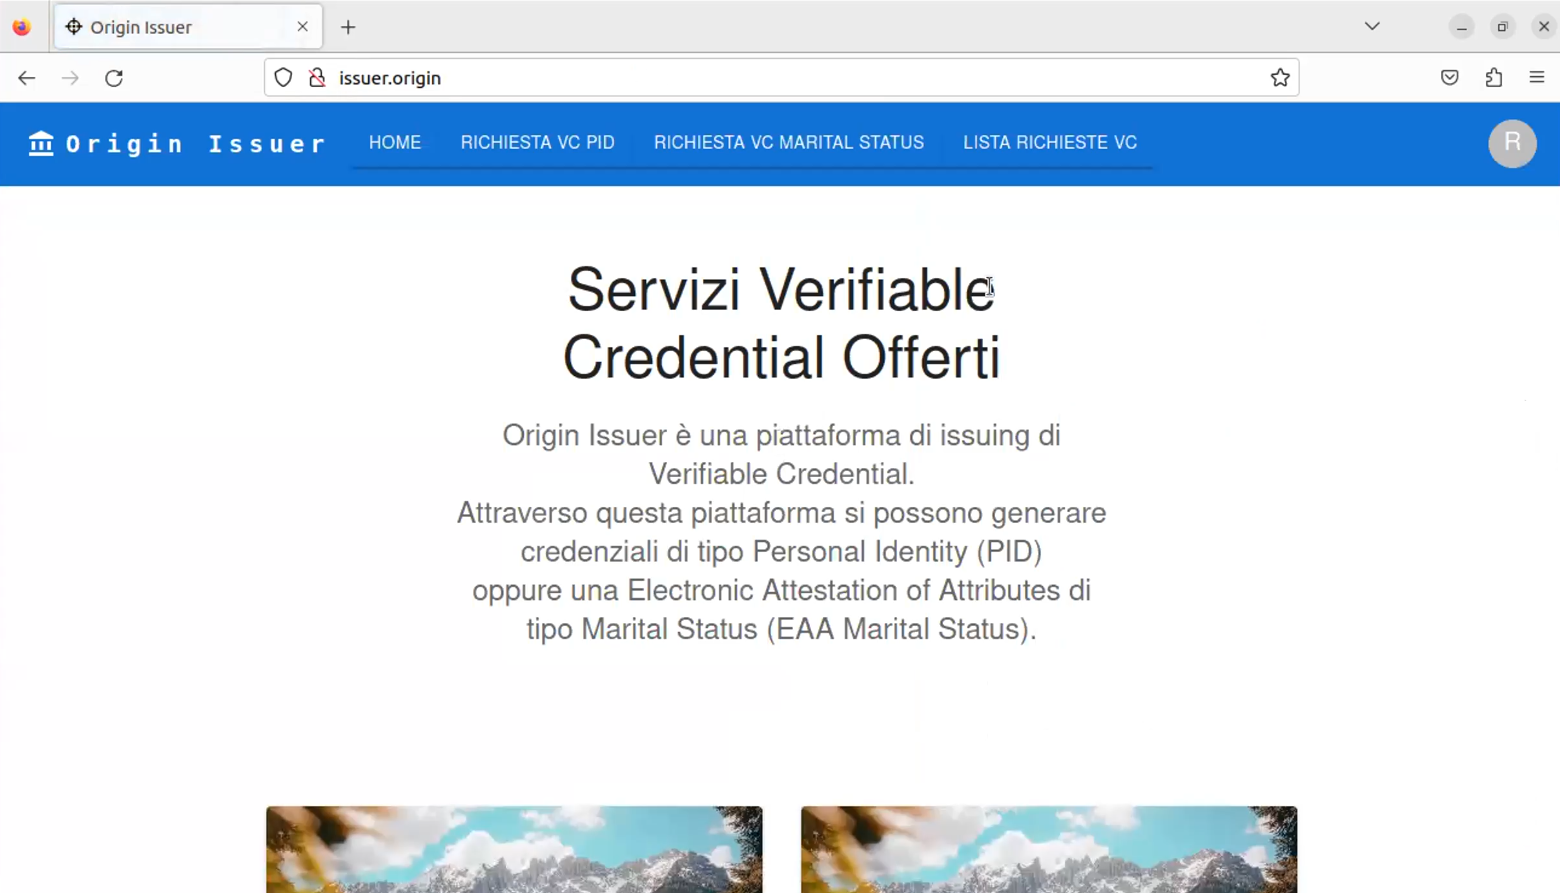
\includegraphics[scale = 0.2]{./res/img/issuer/new/login3.png}
\end{center}



\subsection{Richiesta Credenziale}
\subsubsection{Richiesta PID}
In questa pagina un utente può richiedere una credenziale di tipo \textbf{PID} inserendo i dati richiesti. Una volta inseriti i dati l'utente riceverà un messaggio di conferma e verrà reindirizzato alla lista delle proprie richieste di credenziali.
\begin{center}
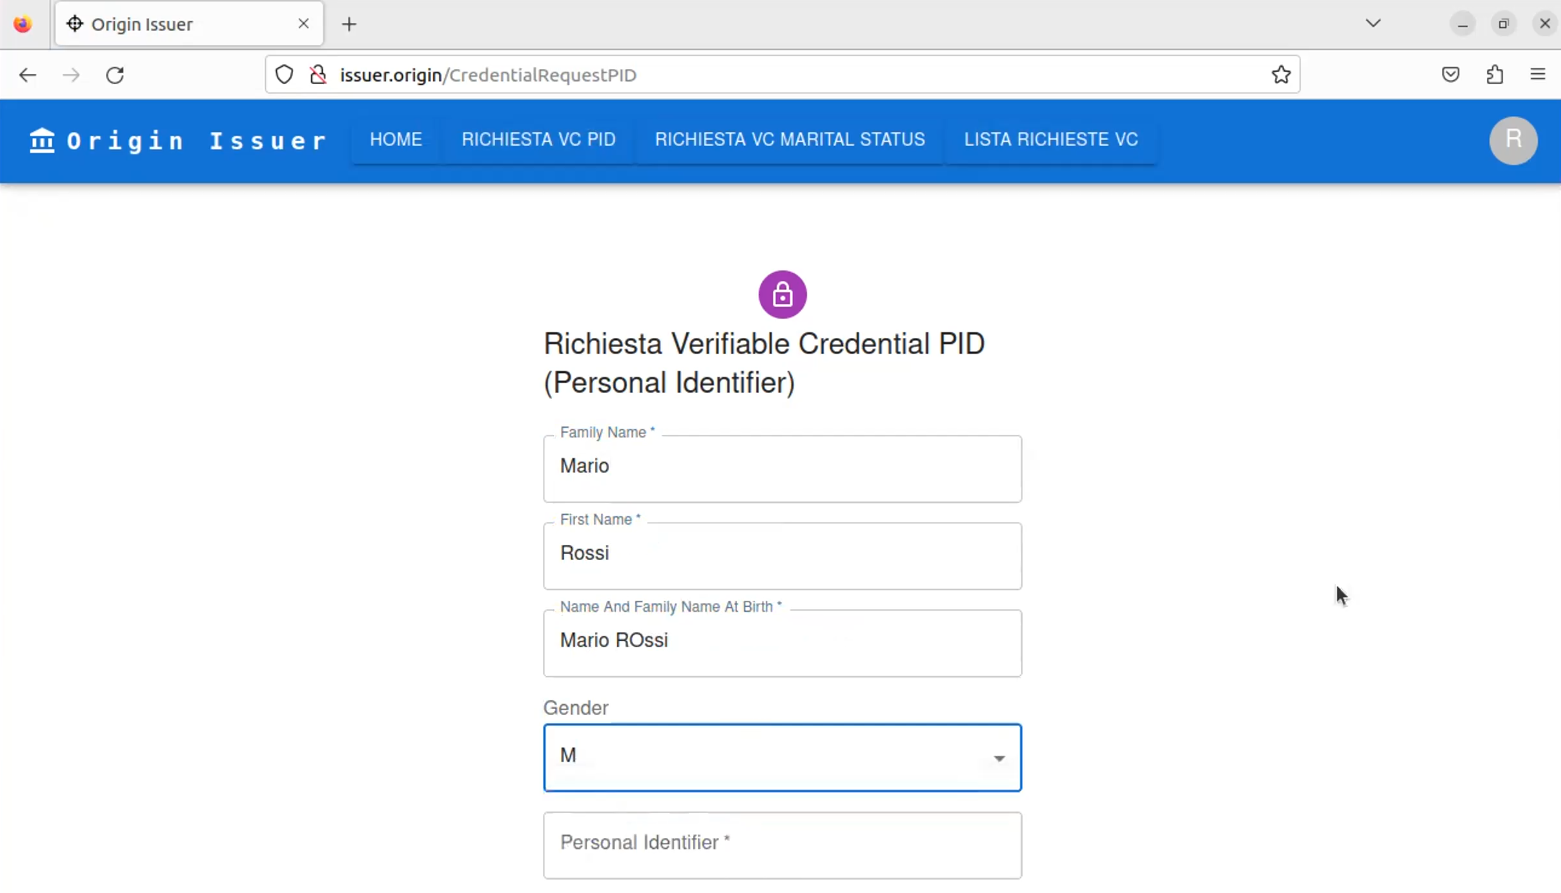
\includegraphics[scale = 0.2]{./res/img/issuer/new/richiestapid1.png}
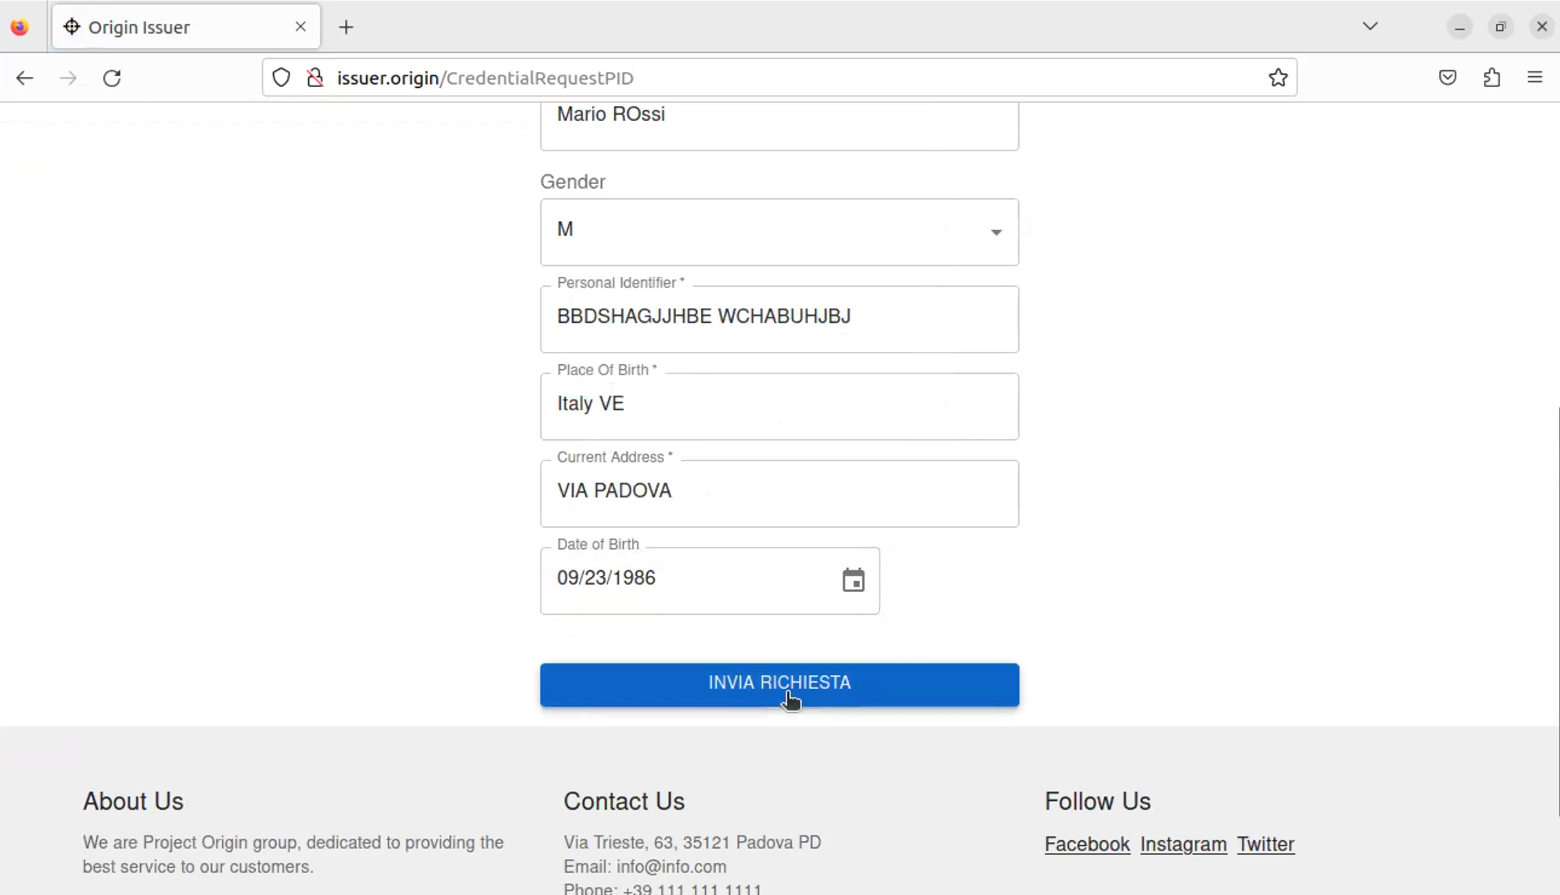
\includegraphics[scale = 0.2]{./res/img/issuer/new/richiestapid2.png}
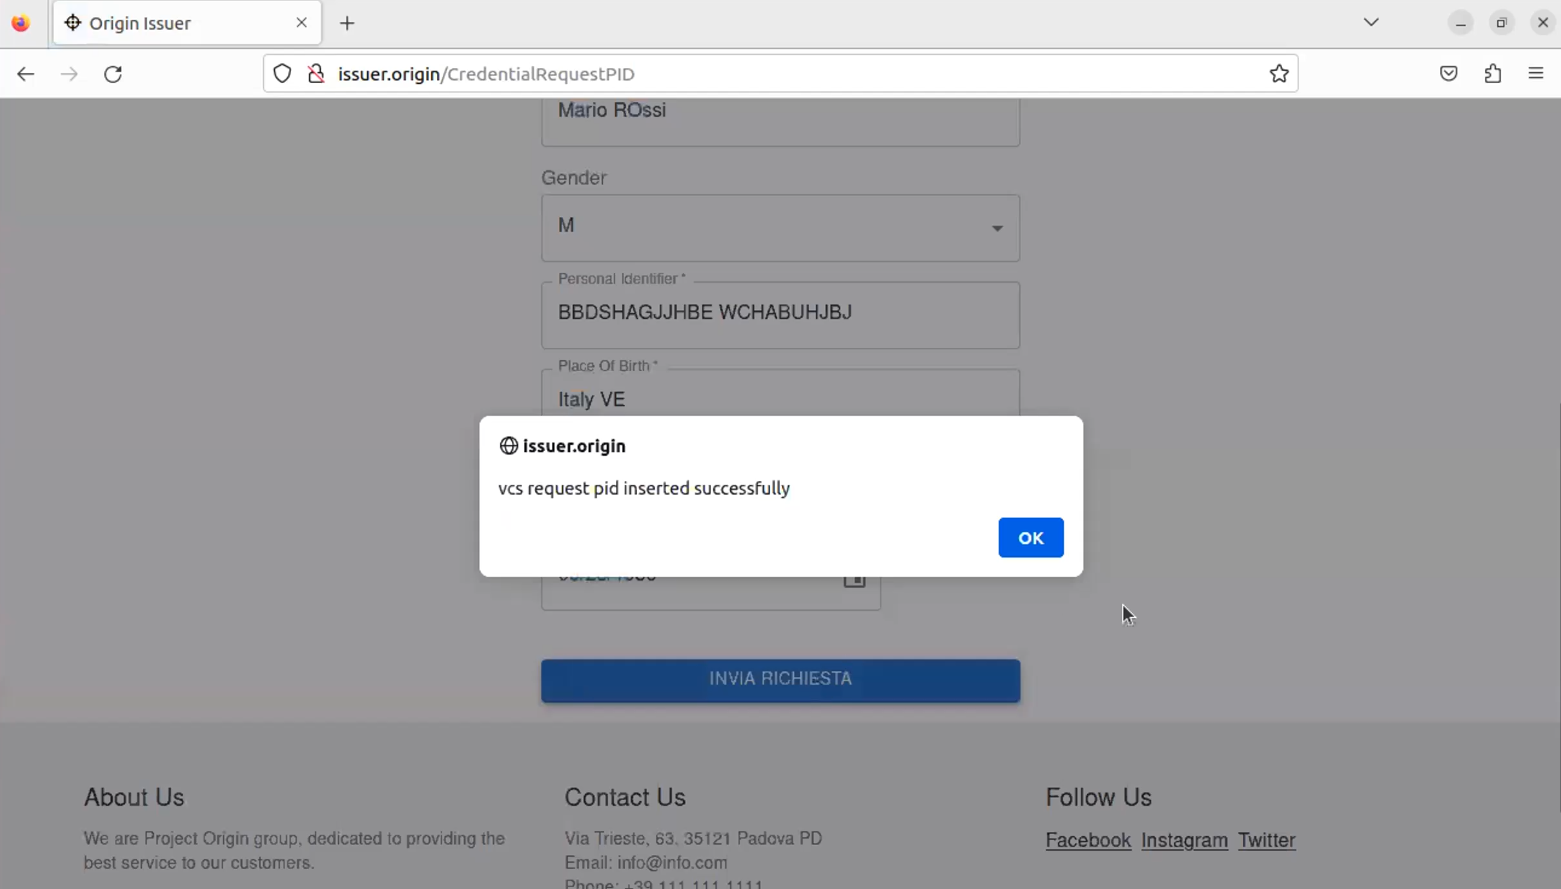
\includegraphics[scale = 0.2]{./res/img/issuer/new/richiestapid3.png}
\end{center}

\subsubsection{Richiesta Marital Status}
In questa pagina un utente può richiedere una credenziale di tipo \textbf{Marital} inserendo i dati richiesti. Una volta inseriti i dati l'utente riceverà un messaggio di conferma e verrà reindirizzato alla lista delle proprie richieste di credenziali.

\subsection{Visualizzazione lista richieste}
\subsubsection{Visualizzazione richieste user} 
In questa pagina l'utente dopo aver fatto una richiesta di credenziale può visualizzare due liste suddivise in PID e Marital. Cliccando su \textbf{Dettaglio} si possono visualizzare tutte le informazioni di una richiesta di credenziale, insieme al suo stato di revisione (In Revisione, Approvato o Rifiutato) e se la credenziale è già stata rilasciata o meno.
\begin{center}
    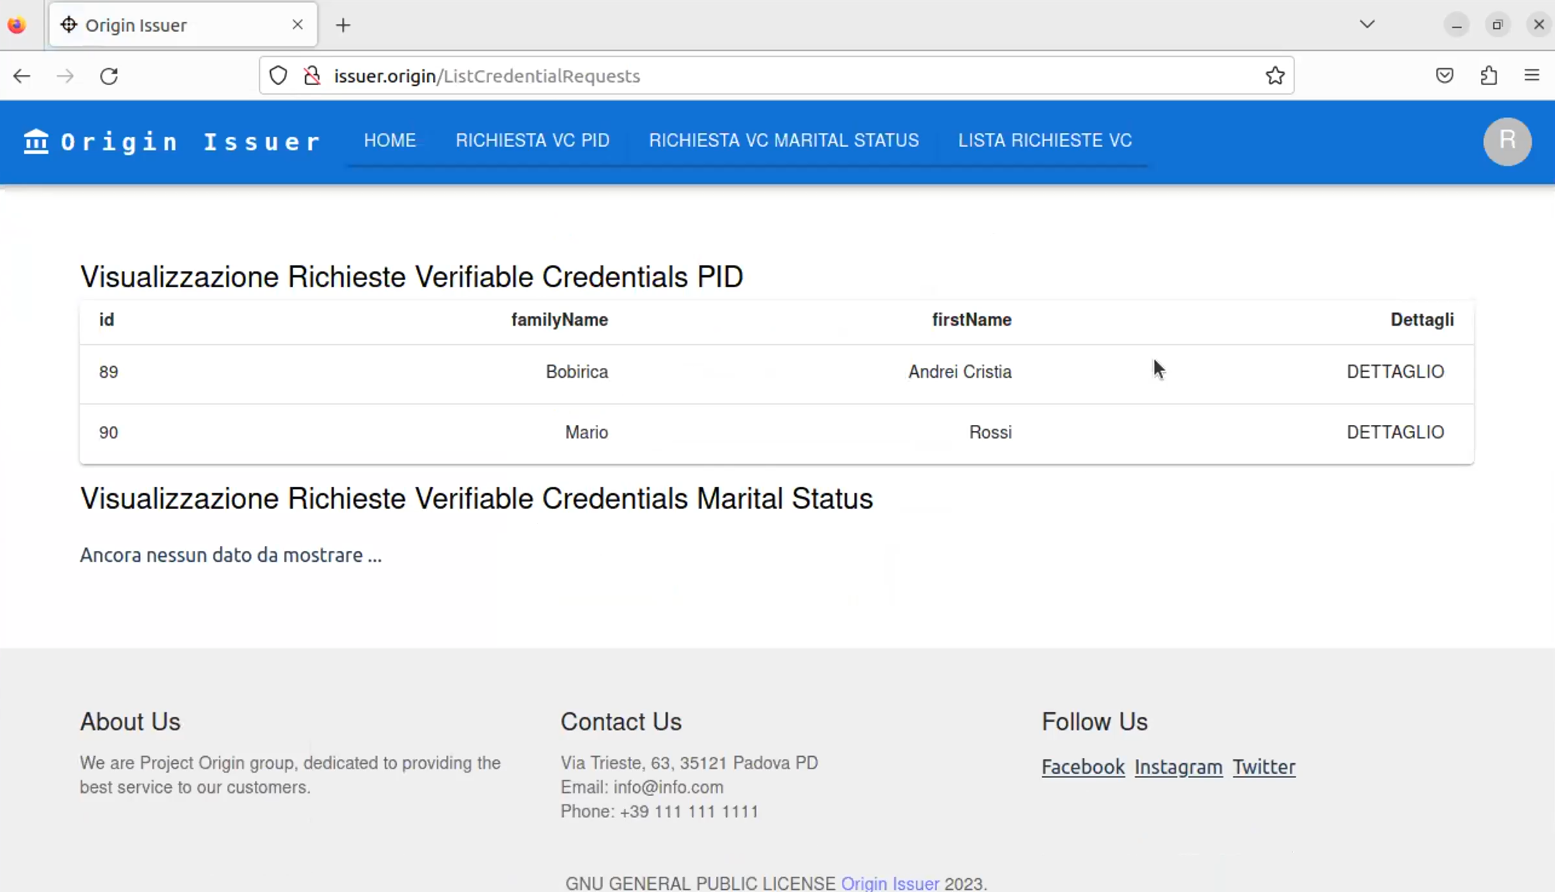
\includegraphics[scale = 0.2]{./res/img/issuer/new/listauser1.png}
    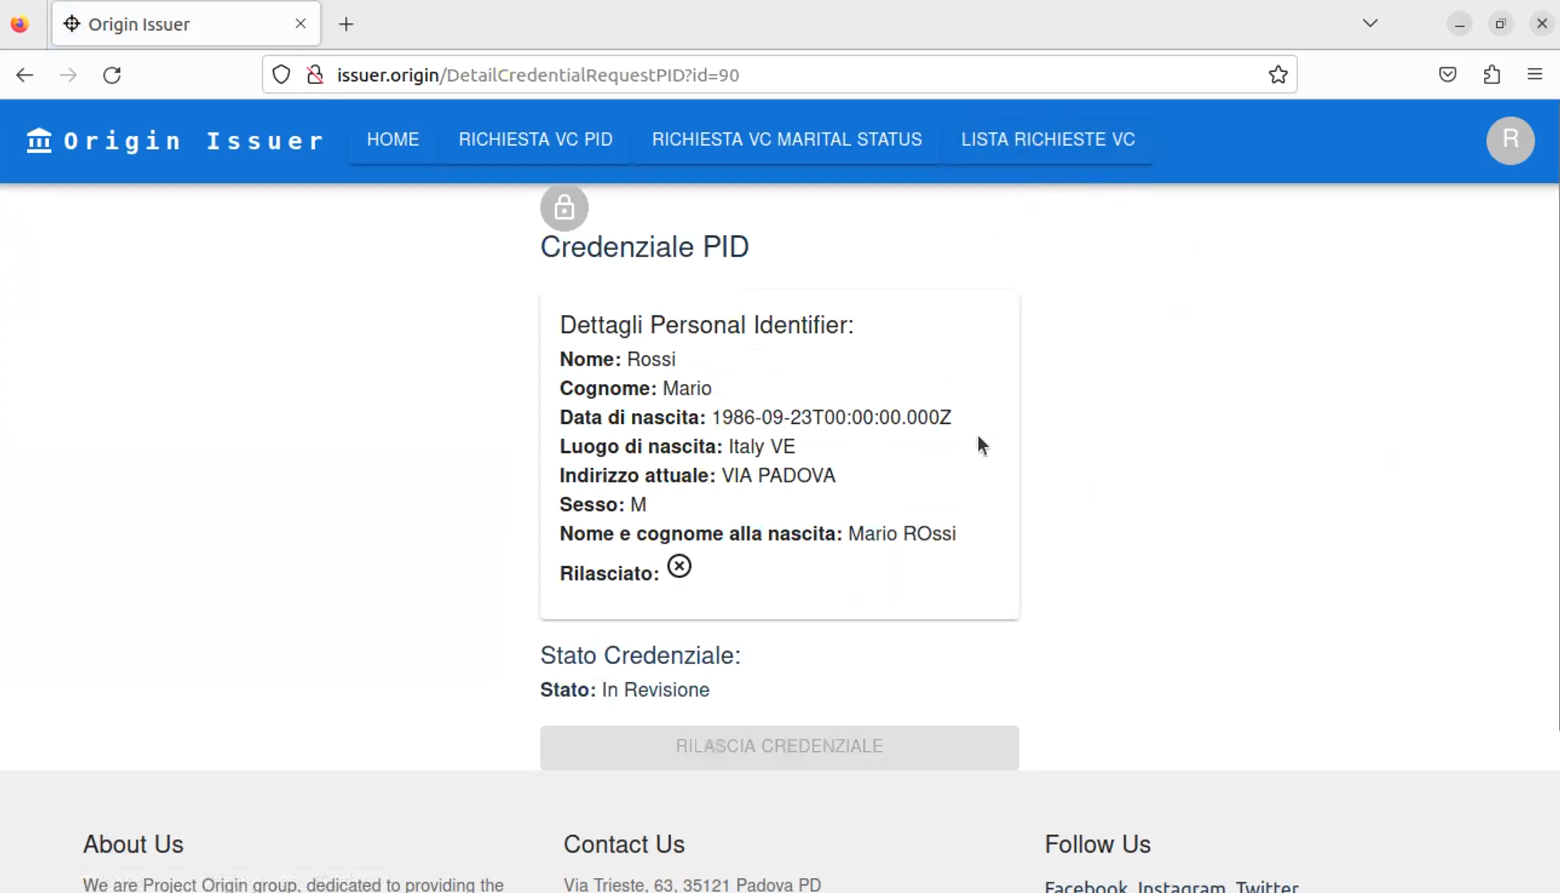
\includegraphics[scale = 0.2]{./res/img/issuer/new/listauser2.png}

\end{center}

\subsection{Rilascio credenziale}
Quando un utente si trova nella pagina di dettaglio di una sua richiesta di credenziale, se la richiesta è stata approvata e la credenziale non è ancora stata rilasciata, l'utente può cliccare sul pulsante Rilascia per rilasciare la credenziale. L'utente può scegliere di rilasciare la credenziale in due maniere: cross device o same device.\\
Inquadrando il codice QR con il proprio wallet si procede con il rilascio in modalità cross device.\\
Per utilizzare la modalità same device si può utilizzare uno dei wallet proposti dall'issuer, come l'Origin Wallet. Successivamente si verrà reindirizzati al wallet.
\begin{center}
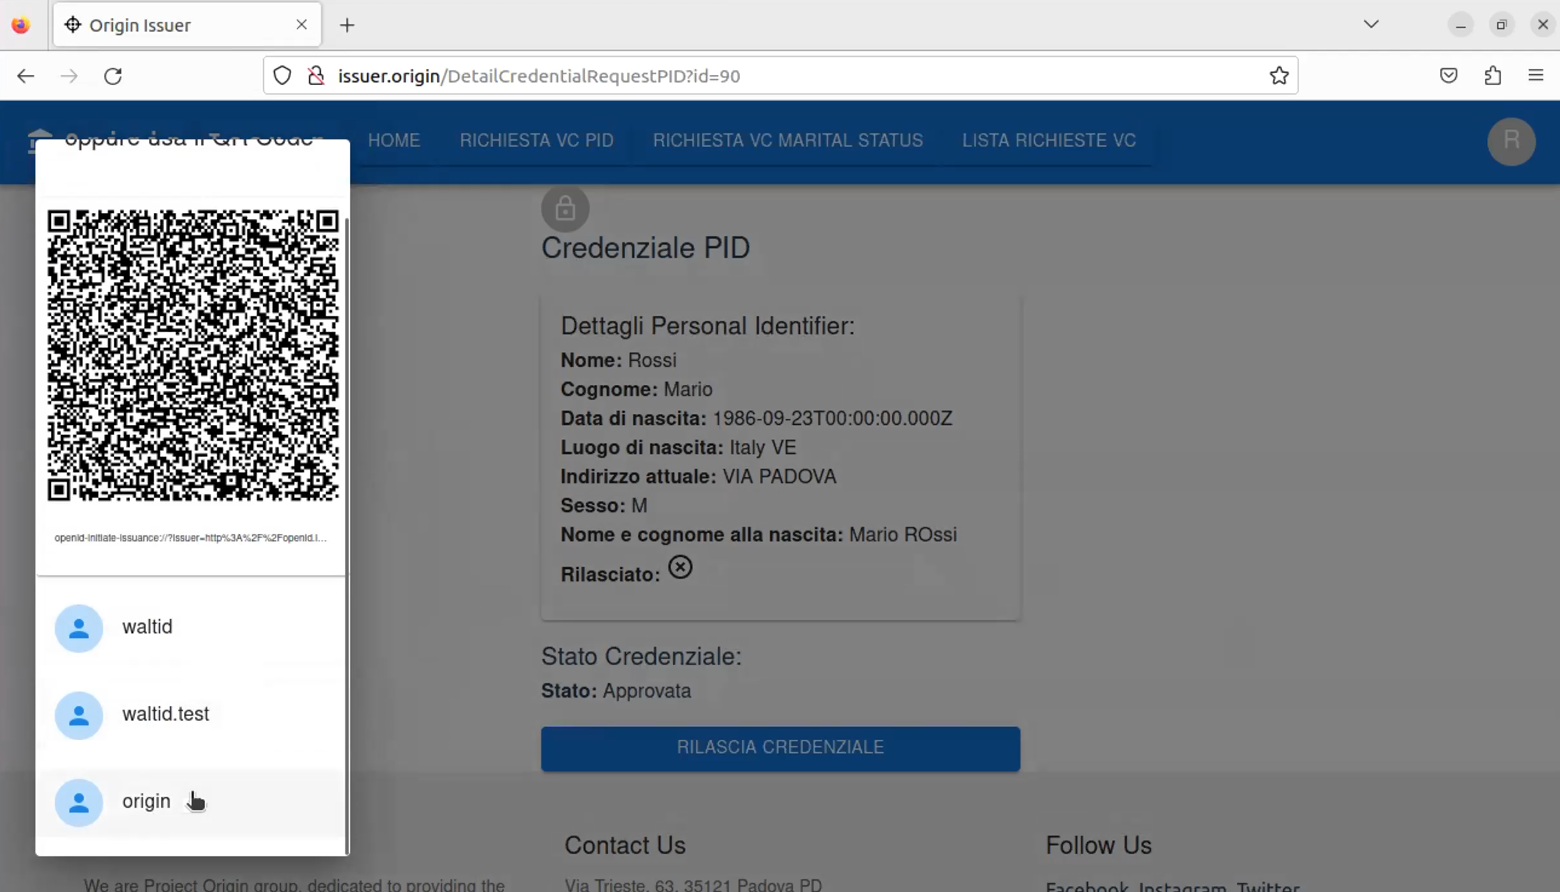
\includegraphics[scale = 0.2]{./res/img/issuer/new/rilascio1.png}  
\end{center}


\subsection{Control Panel Sys Admin}
\subsubsection{Login admin}
In questa pagina un \textbf{admin} può effettuare il login inserendo \textbf{Email} e \textbf{Password} valide. Una volta effettuato il login l'admin verrà reindirizzato alla sua pagina \textbf{Home}.
\begin{center}
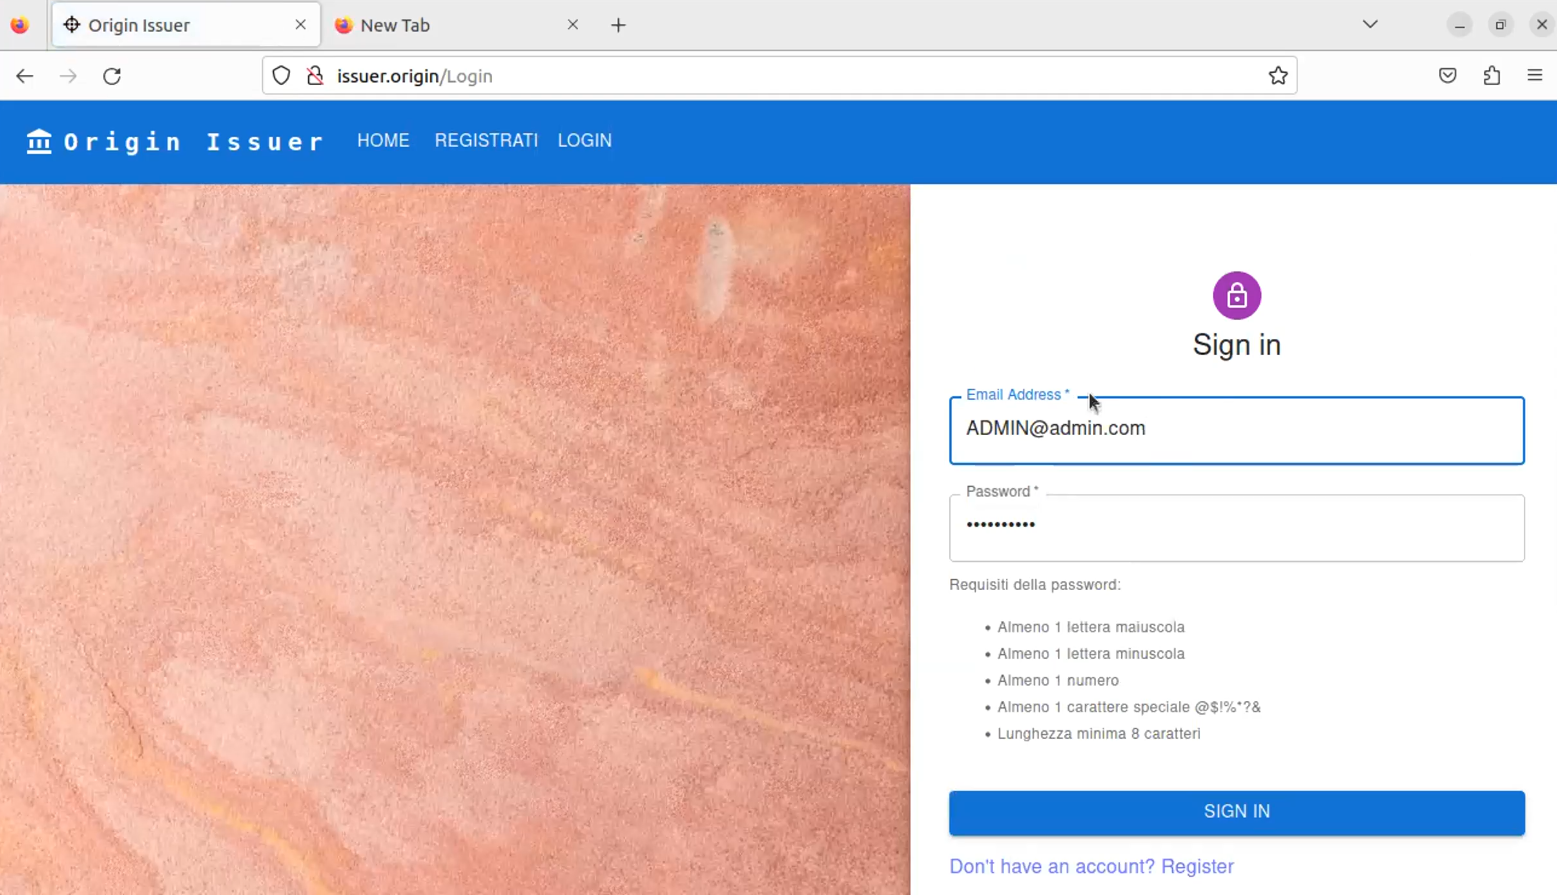
\includegraphics[scale = 0.2]{./res/img/issuer/new/loginadmin1.png}
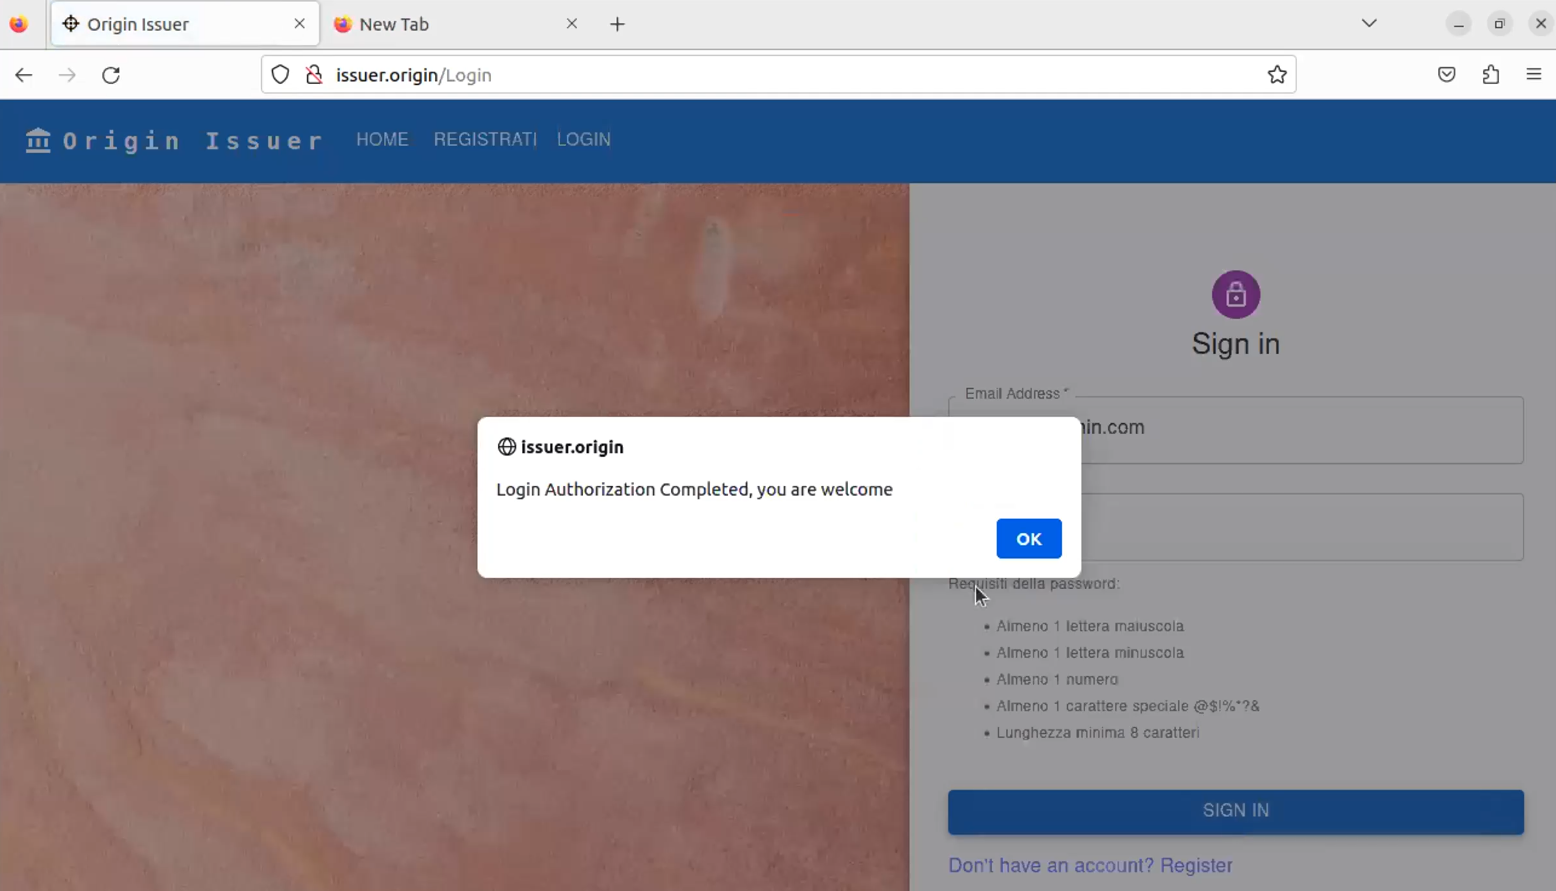
\includegraphics[scale = 0.2]{./res/img/issuer/new/loginadmin2.png}
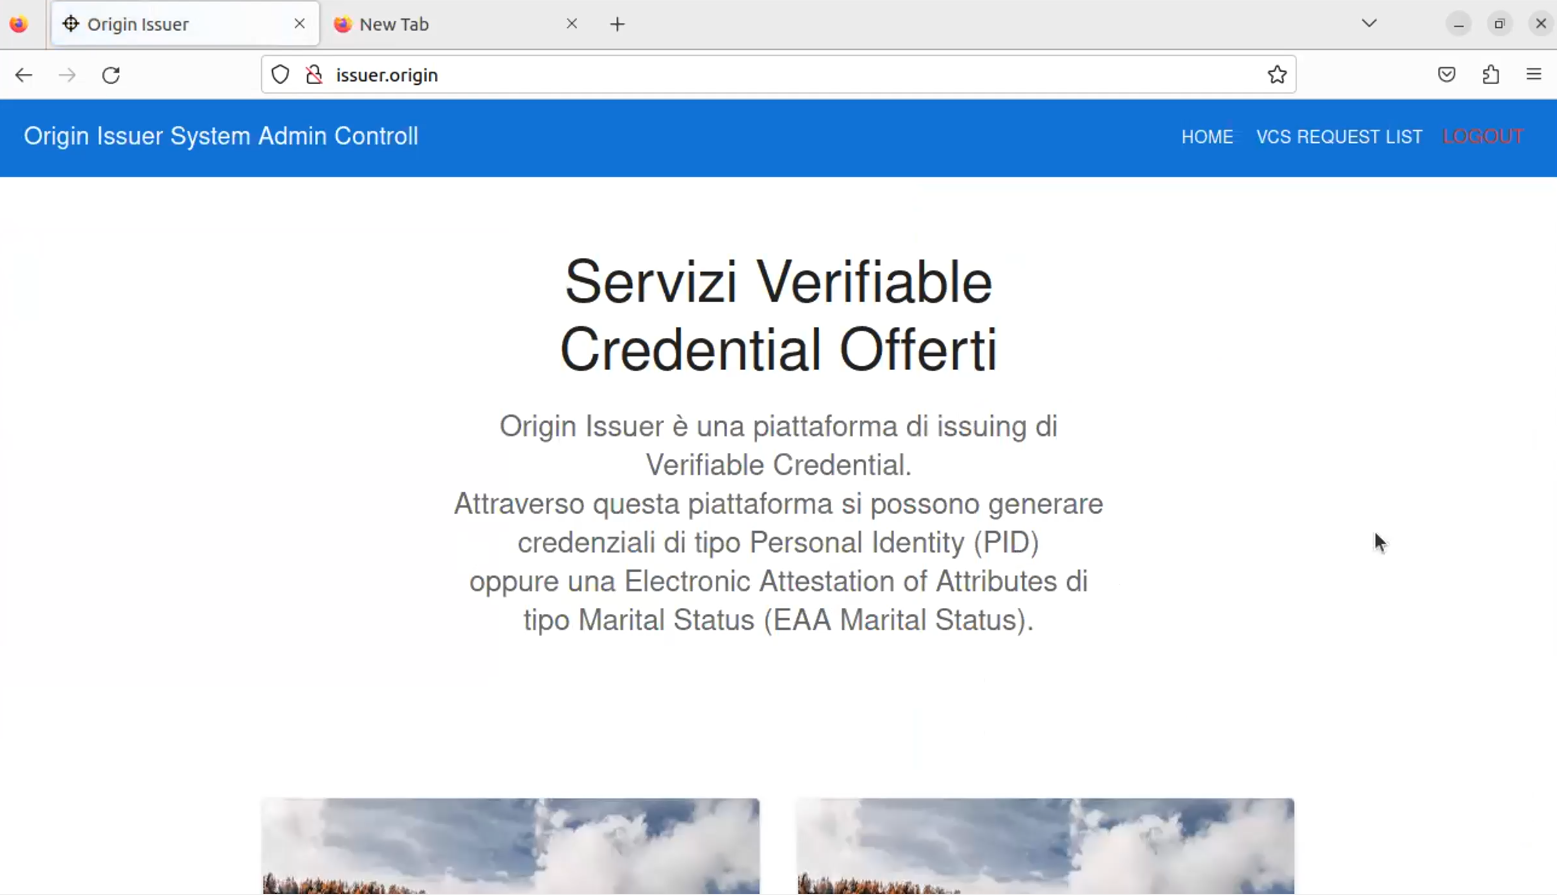
\includegraphics[scale = 0.2]{./res/img/issuer/new/loginadmin3.png}
\end{center}

\subsubsection{Visualizzazione richieste admin e approvazione} 
In questa pagina un admin può visualizzare due liste suddivise in pending e not pending. La lista delle richieste in pending rappresentano le richieste di credenziali non approvate. Cliccando sul pulsante \textbf{Verify} l'admin può approvare o rifiutare la richiesta di credenziale.\\
La lista delle richieste not pending contiene le richieste di credenziali già revisionate, non possono essere modificate.
\begin{center}
    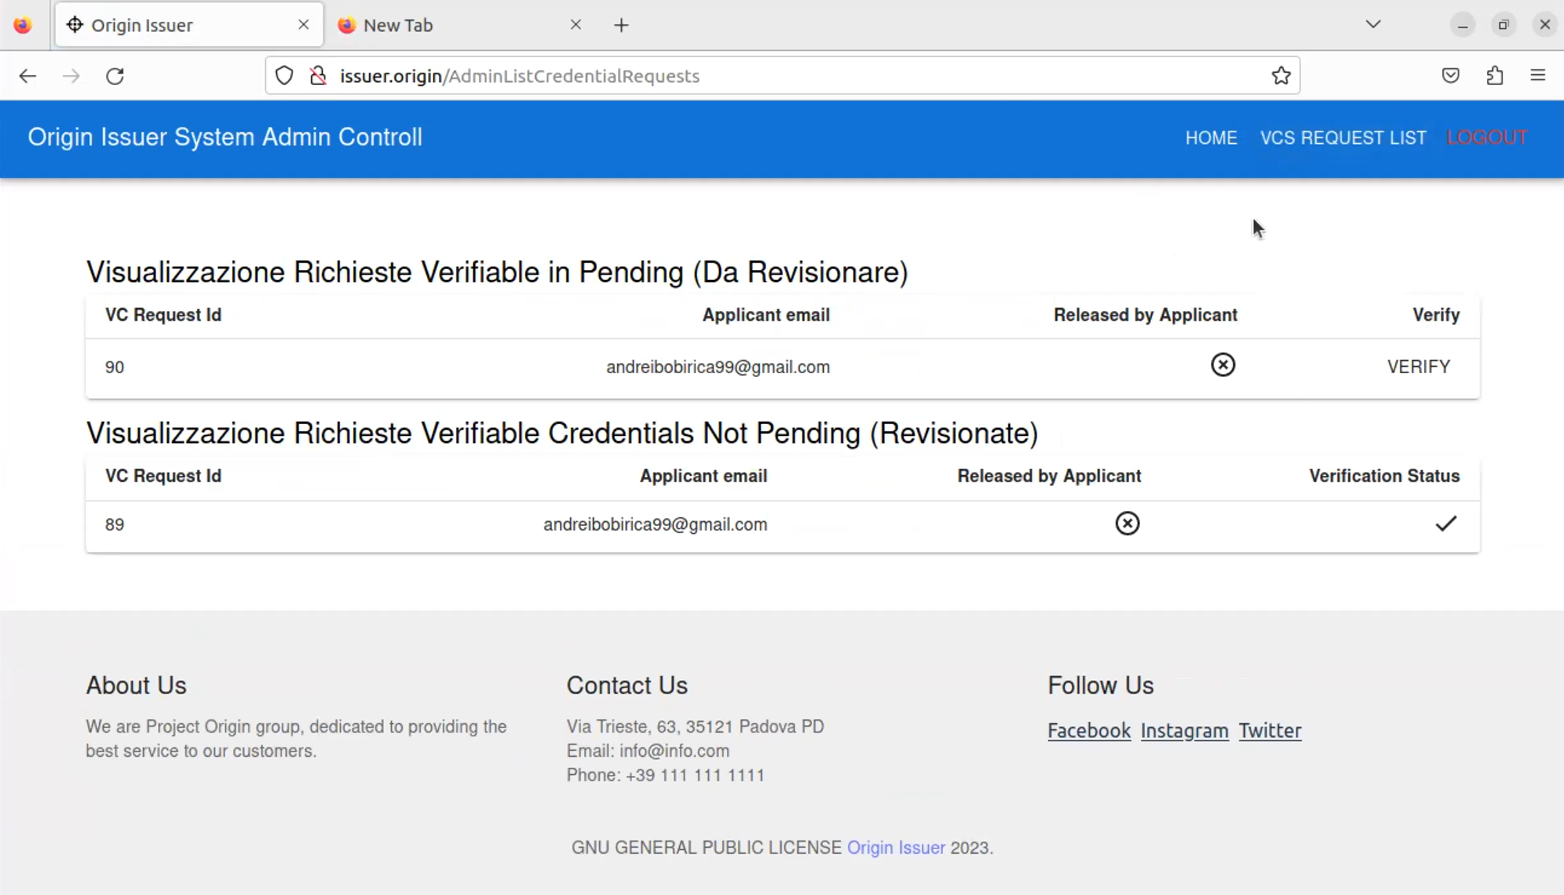
\includegraphics[scale = 0.2]{./res/img/issuer/new/listaadmin1.png}
    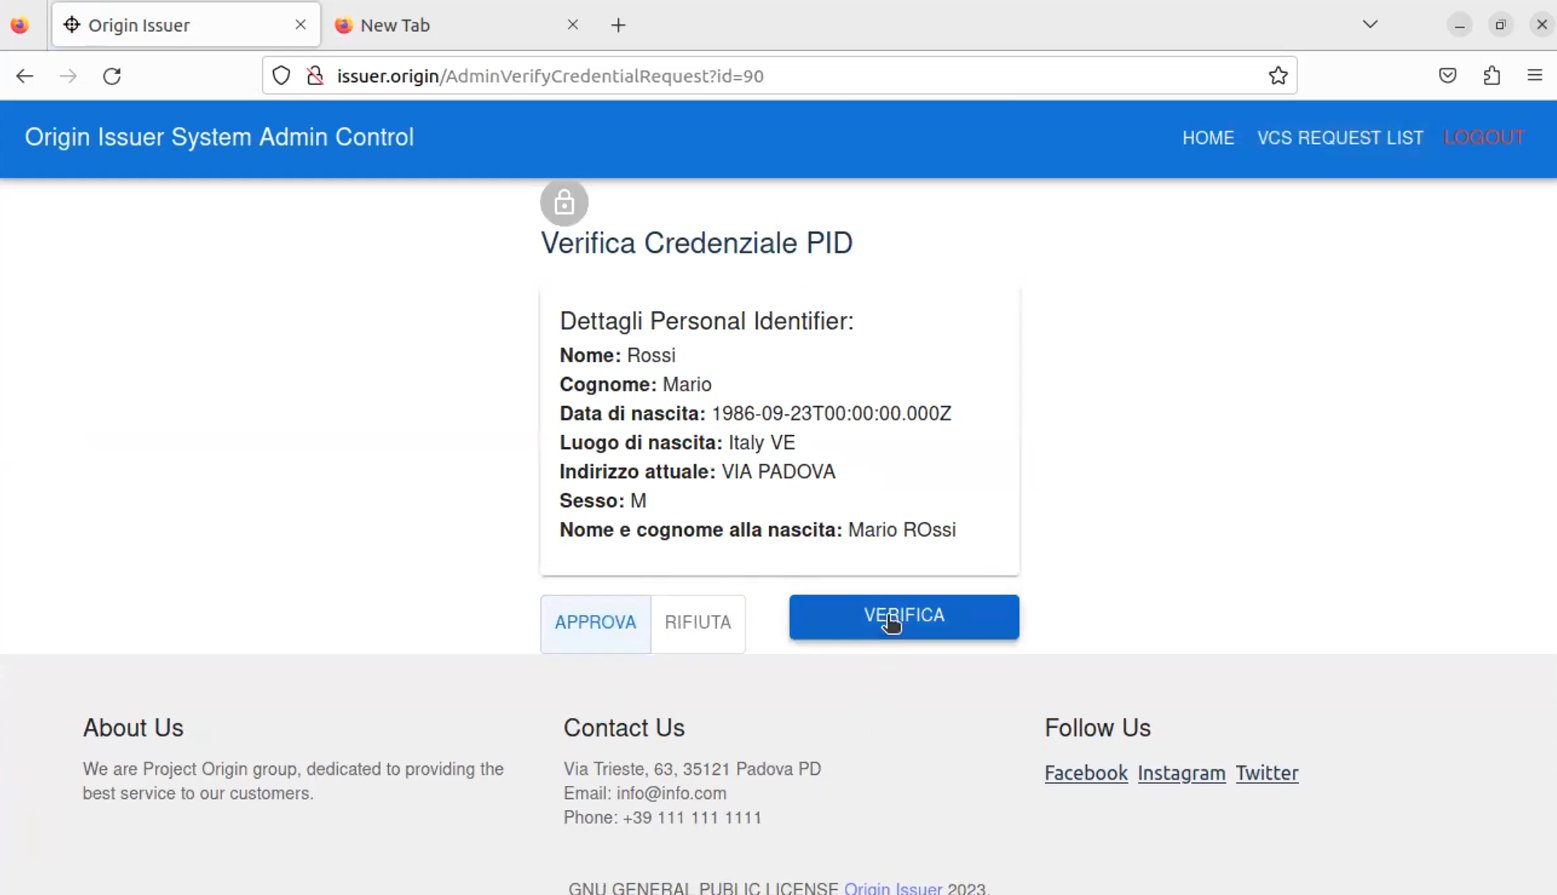
\includegraphics[scale = 0.2]{./res/img/issuer/new/listaadmin2.png}
\end{center}


\clearpage